\documentclass{mini}
\usepackage[utf8]{inputenc}
\usepackage{caption}
\usepackage{subcaption}
\usepackage[polish]{babel}
\usepackage{graphicx}
\usepackage{mathtools}
\usepackage{algpseudocode}
\usepackage{color}
\usepackage{xcolor}
\usepackage{listings}
\usepackage{catchfilebetweentags}
\usepackage{enumitem}

\usepackage{catchfilebetweentags}
\usepackage{etoolbox}
\makeatletter
\patchcmd{\CatchFBT@Fin@l}{\endlinechar\m@ne}{}
  {}{\typeout{Unsuccessful patch!}}
\makeatother

\addto\extraspolish{%  
 \def\figureautorefname{Rysunek}%  
} 

%------------------------------------------------------------------------------%
\title{Realizacje scenariuszy działań}
\author{Robert Jakubowski
\\Hanna Dziegciar
\\Paweł Bielicki
\\Karol Bocian
\\Karol Dzitkowski
\\Mateusz Jankowski
\\Wiktor Ryciuk
\\Mariusz Ambroziak}
\monthyear{\today}
%------------------------------------------------------------------------------%
\begin{document}
%<*tag>

\chapter{Przykłady}

\section{Pytanie czy scenariusz może wystąpić}

	\subsection{Historia}

	\subsection{Opis akcji}

	\subsection{Scenariusz}

	\subsection{Kwerendy}

	\subsection{Analiza}

\section{Pytanie czy dany warunek  zachodzi w danym czasie}

	\subsection{Historia}

	\subsection{Opis akcji}

	\subsection{Scenariusz}

	\subsection{Kwerendy}

	\subsection{Analiza}

\section{Pytanie czy dana akcja jest wykonywana w danym czasie}

	\subsection{Historia}

	\subsection{Opis akcji}
.%Usunąć kropkę - była tylko po to, żeby dobrze strony się wyświetlały - bez niej była lipa
	\subsection{Scenariusz}

	\subsection{Kwerendy}

	\subsection{Analiza}

\section{Pytanie czy cel jest osiągalny}

	\subsection{Historia}

	\subsection{Opis akcji}

	\subsection{Scenariusz}

	\subsection{Kwerendy}

	\subsection{Analiza}

\section{Brak integralnośći}

Przykład \textit{Brak integralnośći} pokazuje scenariusz, który mimo zgodności z warunkami zadania, jest sprzeczny z logiką \textit{common sense} (z powodu braku warunków integralności).

\subsection{Historia}
Mamy Billa oraz kompute. Bill może nacisnąć przycisk \textit{Włącz} lub odłączyć komputer od zasilania. Komputer jest wyłączony i podłączony do zasilania. Jeżeli zostanie naciśnięty jego przycisk \textit{Włącz}, to komputer włącza się.

\subsection{Opis akcji}

\textbf{initially} $\neg on\_computer$  and  $connects\_power\_computer$ \textbf{and} $\neg swithing\_on\_computer$\\
$(click\_button\_on,1)$  \textbf{causes} $switching\_on\_computer$\\
$(click\_button\_on,1)$  \textbf{invokes} $(switch\_on\_computer,2)$  \textbf{after} $1$\\
$(switch\_on\_computer,1)$  \textbf{causes} $on\_computer$\\
$(disconnect\_power,1)$  \textbf{causes} $on\_computer$  \textbf{and} $\neg swithing\_on\_computer$ \\

\subsection{Scenariusz}

\textit{Sc} =$(OBS,ACS)$\\
\textit{OBS} = ${\emptyset}$\\
\textit{ACS}  = ${ 	(click\_button\_on,0+1), (disconnect\_power,)	,3+1),(click\_button\_on,4+1)	}$\\

\subsection{Kwerendy}

\begin{enumerate}
	\item $swithing\_on\_computer$  \textbf{at} $6+2$ \textbf{when} \textit{Sc}
	\item $swithing\_on\_computer$   \textbf{and}  $\neg on\_computer$ \textbf{at} $6+2$ \textit{when} \textbf{Sc}
\end{enumerate}


\subsection{Analiza}
Powyższy scenariusz jest prawidłowy, lecz zawiera pewną niezgodność. W chwili $t = 4+1$ komputer zostaje odcięty od zasilania. Powinien więc wyłączyć się.  Bill chwili $t = 5+1$ naciska przycisk \textit{Włącz}.Komputer zacznie włączać się mimo iż jest odcięty od zasilania. Zachodzą dwa sprzeczne ze sobą stany, tj.  $swithing\_on\_computer = T$  i $on\_computer=T$. Odpowiedzi na powyższe kwerendy będą odpowiednio: $1. True$ i $2. False$. Należy zaznaczyć, że odpowiedzi zgodnie z logiką \textit{commonsense} powinny być sobie równe.

\begin{center}
  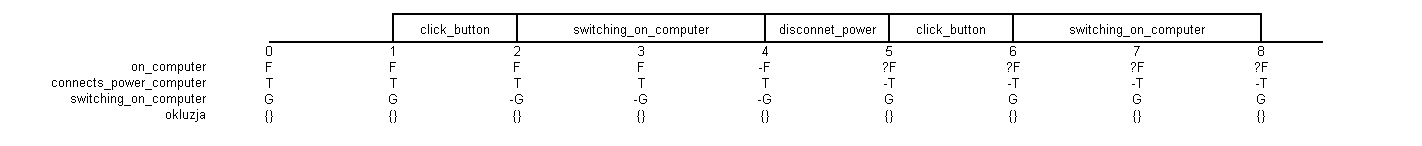
\includegraphics[width=1\textwidth]{Example5}
  \captionof*{figure}{
  }
\end{center}


%</tag>
\end{document}
